\section{Resultate und Diskussion}

Die  berechneten  Werte  sind  als  Tabelle  nochmals  zusammengefasst  (Tabelle
\ref{tab:zusammenfassung}).

Es  war  schwierig, vergleichbare Reibkoeffizienten zu  finden.  Hier  sind  die
beiden        Gleitreibkoeffizienten         verglichen         mit         zwei
Literaturwerten\cite{ref:reibwerte}:

\begin{table}[ht!]
    \begin{center}
        \caption{Zusammenfassung der berechneten Werte}
        \label{tab:zusammenfassung}
        \begin{tabular}{lrrr}
            \toprule
                                    & Gleitreibungskoeffizient & Grenzhaftkraftskoeffizient \\
            \midrule
            Teppich                 & $0.2276 \pm 0.0015$      & $0.3106 \pm 0.0018$        \\
            Plastik                 & $0.1636 \pm 0.0009$      & $0.2890 \pm 0.0013$        \\
            \bottomrule
        \end{tabular}
    \end{center}
\end{table}

\begin{figure}[ht!]
    \centering
    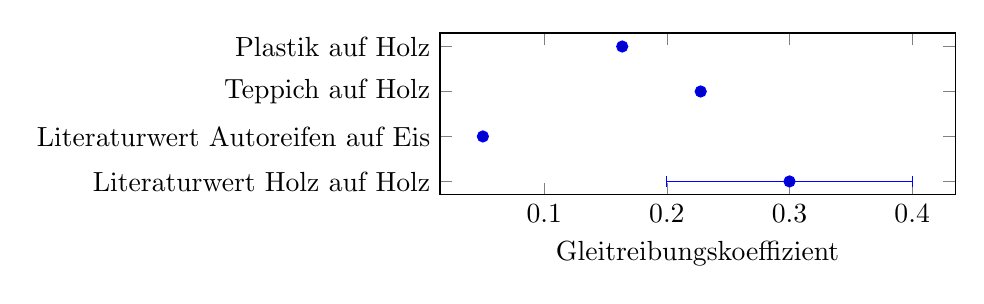
\begin{tikzpicture}
        \begin{axis}[
            width=.67\textwidth,
            height=.3\textwidth,
            xlabel = {Gleitreibungskoeffizient},
            symbolic y coords = {Literaturwert Holz auf Holz,
                                 Literaturwert Autoreifen auf Eis,
                                 Teppich auf Holz,
                                 Plastik auf Holz},
        ]
        \addplot+[
            only marks,error bars/.cd,
            x dir=both,x explicit,
            error bar style={line width=0.5pt},
            ]
        coordinates {
            (0.30,Literaturwert Holz auf Holz)         +- (0.10,0)
            (0.05,Literaturwert Autoreifen auf Eis)
            (0.2276,Teppich auf Holz)                  +- (0.0015,0)
            (0.1636,Plastik auf Holz)                  +- (0.0009,0)
        };
        \end{axis}
    \end{tikzpicture}
    \caption{Grafische Darstellung der Grenzhaftkoeffizienten und Vergleich mit ein paar Literaturwerten}
    \label{fig:gleitreibungskraft}
\end{figure}

Und  hier  sind   die  beiden  Grenzhaftkoeffizienten  nochmals  verglichen  mit
Literaturwerten\cite{ref:reibwerte}:

\begin{figure}[ht!]
    \centering
    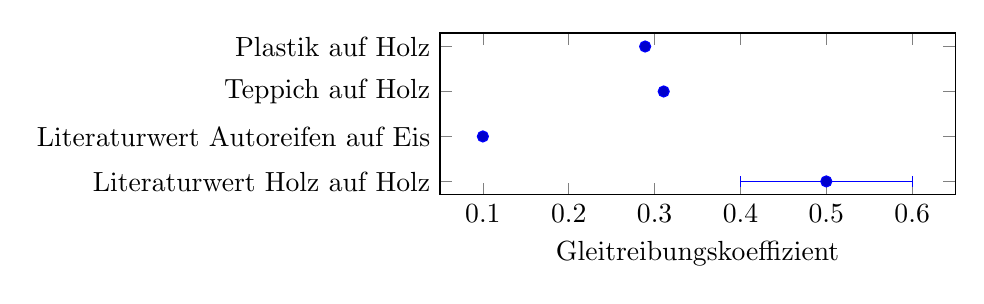
\begin{tikzpicture}
        \begin{axis}[
            width=.67\textwidth,
            height=.3\textwidth,
            xlabel = {Gleitreibungskoeffizient},
            symbolic y coords = {Literaturwert Holz auf Holz,
                                 Literaturwert Autoreifen auf Eis,
                                 Teppich auf Holz,
                                 Plastik auf Holz},
        ]
        \addplot+[
            only marks,error bars/.cd,
            x dir=both,x explicit,
            error bar style={line width=0.5pt},
            ]
        coordinates {
            (0.50,Literaturwert Holz auf Holz)         +- (0.10,0)
            (0.10,Literaturwert Autoreifen auf Eis)
            (0.3106,Teppich auf Holz)                  +- (0.0018,0)
            (0.2890,Plastik auf Holz)                  +- (0.0013,0)
        };
        \end{axis}
    \end{tikzpicture}
    \caption{Grafische Darstellung der Gleitreibungskoeffizienten und Vergleich mit ein paar Literaturwerten}
    \label{fig:grenzhaftkraft}
\end{figure}

Die  berechneten Koeffizienten scheinen vern\"umftig zu  sein.  Die  berechneten
Fehler,  jedoch,  k\"onnen  niemals so genau sein.  Es  ist  offensichtlich  ein
systematischer  Fehler  vorhanden,  n\"amlich die spezifische Eigenschaften  der
Bahn, die Eigenschaften des ausgew\"ahlten  Teppichs/Plastiks,  die  Temperatur,
Feuchtigkeit, Alter der Vorrichtung usw.

W\"urde  das  Experiment  mit  einer anderen Vorrichtung wiederholt  werden,  so
w\"urden    sehr    wahrscheinlich   ganz   andere   Koeffizienten    entstehen.


